\justifying

The Sun is our nearest astrophysical object, which serves as a natural laboratory for various branches of Physics - atomic physics, spectroscopy, turbulence, magneto-hydrodynamics, stellar evolution, dynamo and magnetism and plays a key role in space and terrestrial weather. The Sun is also the primary source of light and energy on Earth. So it is only natural that we try to understand the different physical processes involved in the energetics of the Sun, which directly affects life on Earth. In this chapter, I briefly introduce the Sun, various layers of its atmosphere and solar flares. Finally, we provide a motivation for the thesis and a brief outline.

%%%%%%%%%%%%%%%%%%%%%%%%%
\section{The Sun}\label{Sun}
%%%%%%%%%%%%%%%%%%%%%%%%%

The Sun is a G2V star, with surface luminosity $3.86~\times~10^{26}$~W and an effective temperature of $\sim 5780~K$. The Sun is mostly made out of Hydrogen (92.1\%) and Helium (7.8\%), along with negligible quantities of heavier elements C, N, O, Mg, Si, Ne and Fe, among others. The study of the Sun can be divided into three components, \textit{viz.} the solar interior, the solar atmosphere and the Heliosphere. Fig.~\ref{fig_solar_int} shows a schematic diagram of various regions of the Sun. Below, we briefly describe these three regions.

%%%%%%%%%%%%%%%%%%%%%%%%%
\section{The Solar Interior}\label{solar_int} 
%%%%%%%%%%%%%%%%%%%%%%%%%

Depending on various physical characteristics, the solar interior can be divided into three zones {\it e.g.} the core, radiative zone and convective zone. In the innermost zone, the core, the Sun has a temperature of about 15~MK and a density of $\mathrm{1.6\times 10^{5}~km.m^{-3}}$. Here Hydrogen fuses into Helium primarily by p-p chain reaction \citep{bethe38} and to some extent by CNO cycle \citep{bethe39}. Beyond the core, we have the optically thick radiative zone, where the Hydrogen and Helium are completely ionized due to very high density. The high energy $\gamma$-ray photons generated in the core have a very small mean free path in this region, as they collide numerous times and propagate across this region. As we move radially outwards, temperature and density both decrease slowly due to gravitational equilibrium. Due to this reduction of temperature, there is a decrease in the thermal motion of the particles, and the hydrogen and helium start to recombine, giving rise to an increase in opacity at the top of the radiative zone. This change in opacity makes the propagation of photons via radiation less efficient, as photons get trapped and reabsorbed more. This creates a sharp temperature gradient due to the "photon pileup". This temperature gradient gives rise "convective instability". This is the convective zone where the energy from the inner layers of the Sun is transported adiabatically to the surface of the Sun.
%In between the radiative and the convective zone, there is \sroy{believed to be }a thin layer, roughly at $\sim~0.7~R_{\odot}$ known as the tachocline. \sroy{This region} is believed to play a major role in generating Sun's magnetic field via the Dynamo process \citep{corbard01}.

%% ############# %%
\begin{figure}[ht!]
    \centering
    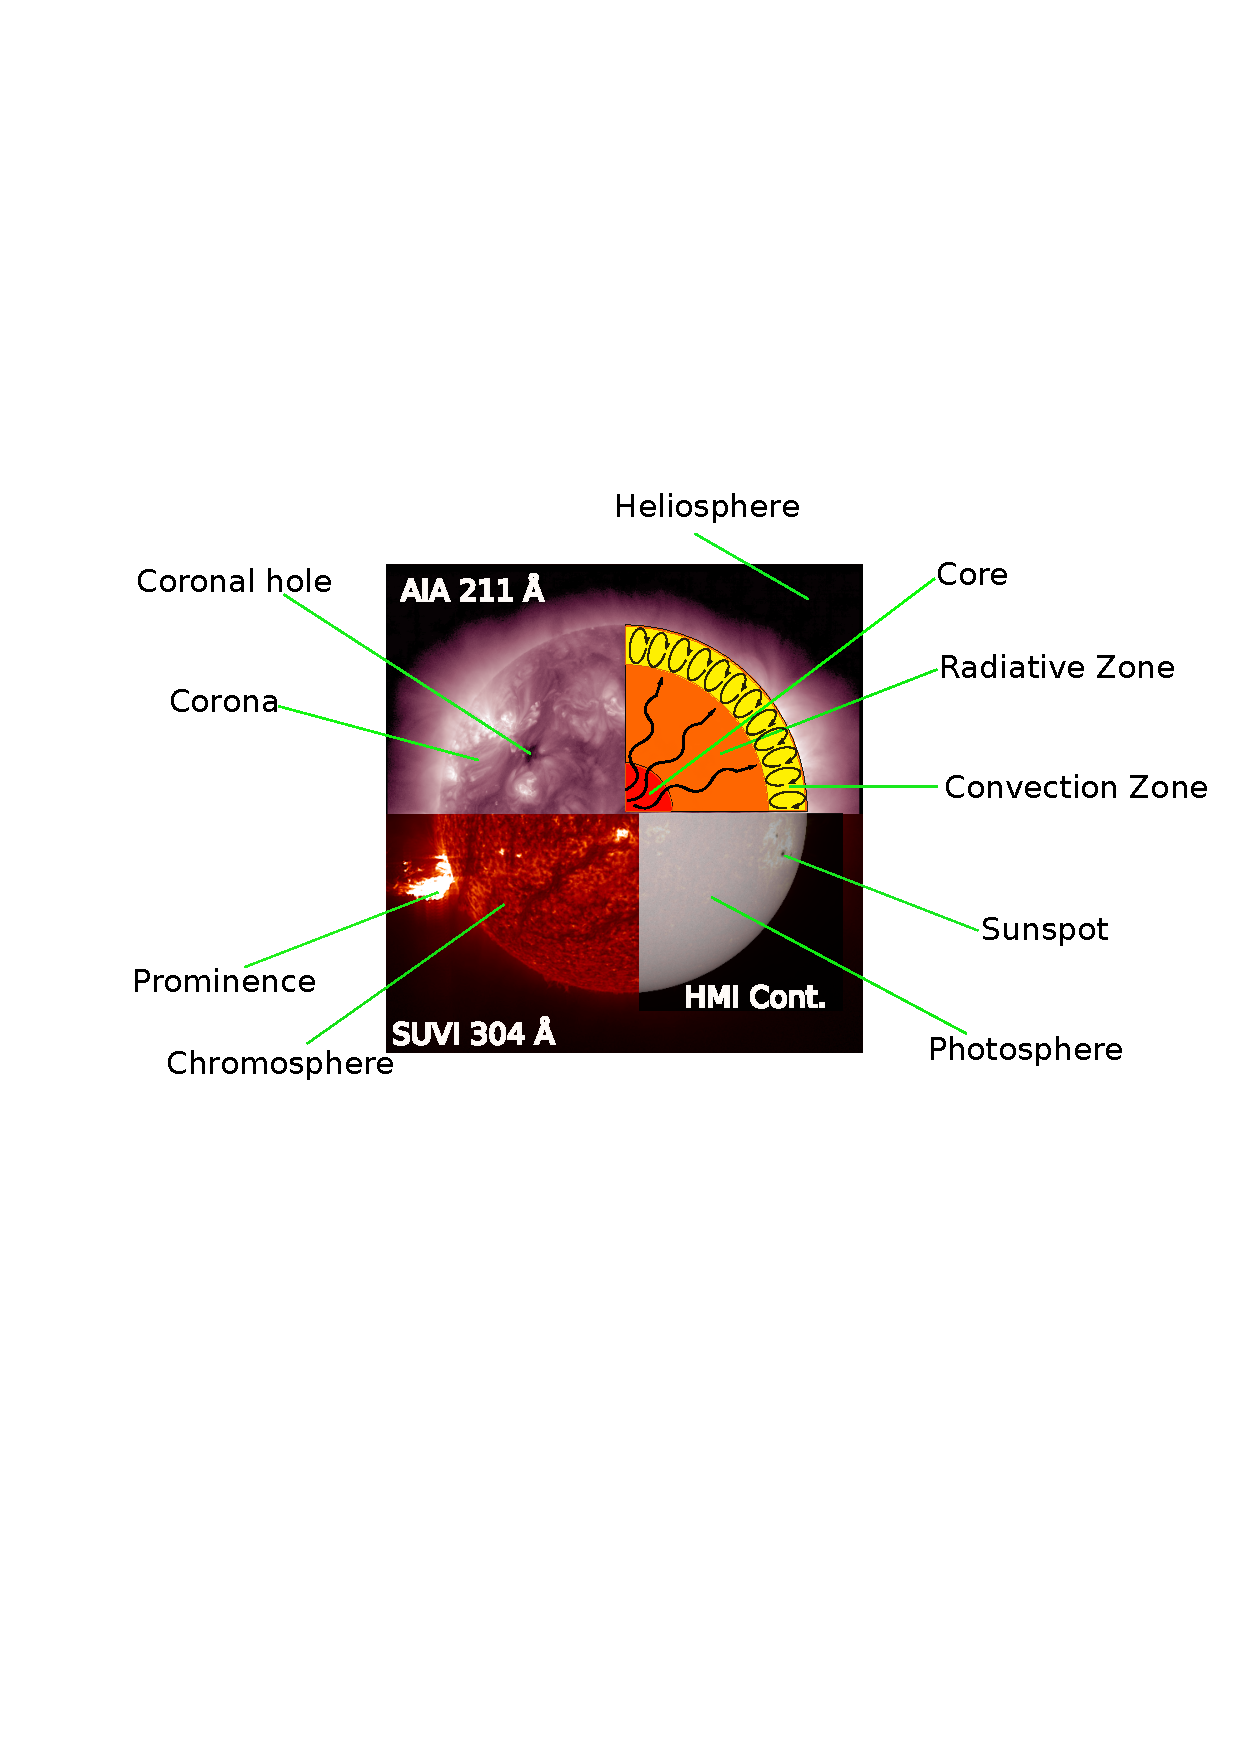
\includegraphics[trim={2cm 11cm 0.5cm 8cm}, clip, width=0.9\textwidth]{solar_int.pdf}
    \caption[A schematic depiction of the different regions of the Sun.]{A schematic depiction of the different regions of the Sun, including some of the most prominent magnetic structures on the Sun e.g., Sunspot, prominence, coronal hole.}
    \label{fig_solar_int}
\end{figure}
%% ############# %% 

The core and the radiative zone of the Sun rotate as a solid body, whereas the convective zone rotates deferentially. The rotation period varies from $\sim~25~days$ to $\sim~35~days$ from the equator to the pole.

%%%%%%%%%%%%%%%%%%%%%%%%%%%%%
\section{The Solar Atmosphere}\label{solar_atmos}
%%%%%%%%%%%%%%%%%%%%%%%%%%%%%

The layers outside the convection zone together form the solar atmosphere and is further divided into different regions. The photosphere, which is also known as the Sun's surface, the chromosphere, the transition region and the corona. While we can define geometrical height or depths to define these layers, it is much more useful to define them using the local optical depths of various spectral lines, which are directly used to observe the layers. This also gives us an idea about which spectral features originate mainly from which portions of the solar atmosphere. Fig.~\ref{fig_solar_atm} shows the variation of temperature and number density across various layers of the solar atmosphere \citep{philips08}. 

%% ############# %%
\begin{figure}[ht!]
    \centering
    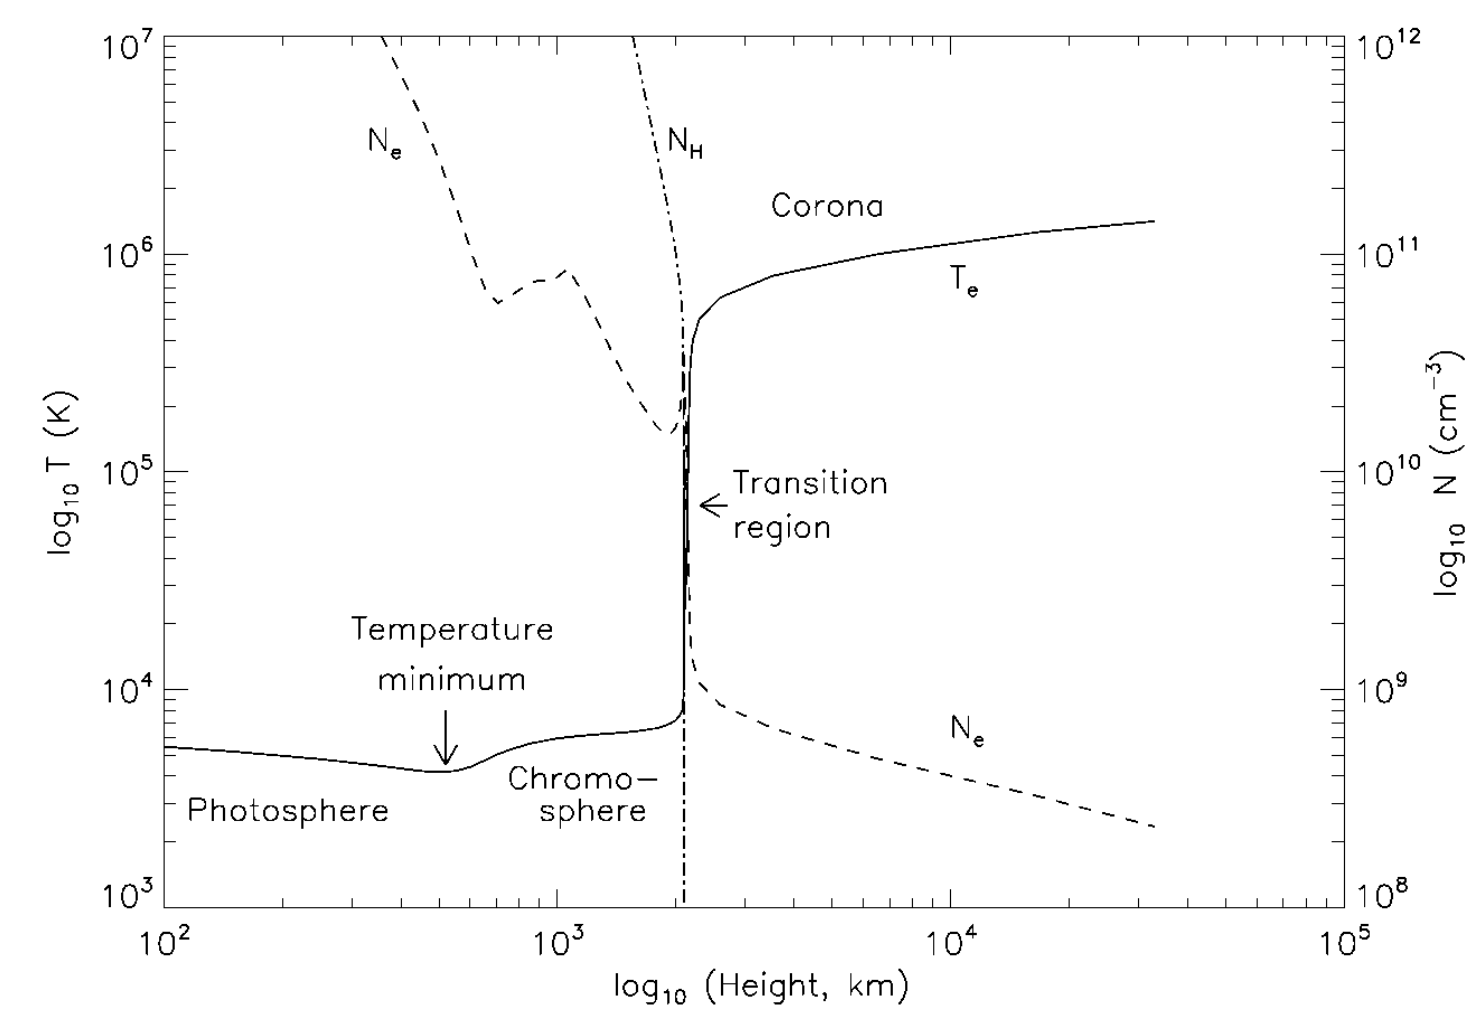
\includegraphics[width = 0.8\linewidth]{Figures/solar_atm.png}
    \caption[Density and temperature profiles across various layers of the Sun.]{The variation of electron temperature (solid line) and electron density ($\mathrm{N_{e}}$, dashed line) and density of neutral hydrogen atoms ($\mathrm{N_{H}}$, dot-dashed line) in the solar atmosphere \citep{philips08}.}
    \label{fig_solar_atm}
\end{figure}
%% ############# %%

%%%%%%%%%%%%%%%%%%%%%%%%%%%%%%%%%%%%%%%%%%%%%%%%%%%%%%%
\subsection{The Photosphere}\label{photosphere}
%%%%%%%%%%%%%%%%%%%%%%%%%%%%%%%%%%%%%%%%%%%%%%%%%%%%%%%

The photosphere is defined to be the layer where $\tau_{\lambda~\sim~5500}=1$. This is in the green part of the visible spectrum and the Sun is opaque in visible beyond this layer, hence it is called to be the surface of the Sun. This layer is 400{--}600~km thick and has an effective temperature of $\sim$5780~K. The magnetic field lines arising from the tachocline penetrate the photosphere and create a `carpet' over the whole region \citep{priest14}. As mentioned earlier, this is the solar surface known as the `quiet Sun' (QS). This region exhibits an average magnetic flux density of 10{--}50 G. The QS surface is covered with cells of roughly four sizes, namely, granules, mesogranules, supergranules and giant cells.

Some regions exhibit much stronger magnetic flux density, often associated with highly twisted magnetic field structures. These magnetic features are manifested as Sunspots. The Sunspots harbour some of the strongest concentrated magnetic fields, reaching up to several kilogauss in strength. The other noteworthy solar magnetic structure apart from these are believed to be spatially unresolved flux tubes composing a network with field strengths $\sim$ {\it $O(10^{3} G)$}\citep{solanki93,grossman96,rubio19}.

As the density changes drastically at the photosphere compared to the convective zone, the thermalized photons from the Sun's core start free streaming, as the mean free path also increases drastically and, as a result, perturbs the thermal equilibrium (TE). Therefore, the thermodynamic quantities of the photosphere are defined under the assumption of Local Thermal Equilibrium (LTE). As we move higher from the photosphere, the LTE conditions also start deviating because the density keeps on decreasing steadily \citep{philips08}.

%%%%%%%%%%%%%%%%%%%%%%%%%%%%%
\subsection{The Chromosphere}\label{chromosphere}
%%%%%%%%%%%%%%%%%%%%%%%%%%%%%

The chromosphere is a highly non-uniform dynamic layer with a thickness of 1500{--}3000~km, with increasing temperature (up to $10^{4}$ K) and decreasing number density. As seen in Fig.~\ref{fig_solar_atm}, the temperature of the chromosphere saturates before the dramatic rise in the transition region. This saturation is attributed to a steady deposition of acoustic energy by the creation of shock waves \citep{carlsson07}. The chromosphere also exhibits a sharp gradient in the plasma $\beta$ factor, non-LTE conditions, and the dominance of wave motions. The observable features in the chromosphere are active regions, sunspots, plages and also light bridges as labelled in images taken by IRIS SJI (slit-jaw imager) 2796 {\AA} (left panel) and 2832 {\AA} (right panel) displayed in Fig.~\ref{fig:sji_features}.  

%%%%%%%%%%%%%%%%
\begin{figure}[ht!]
    \centering
    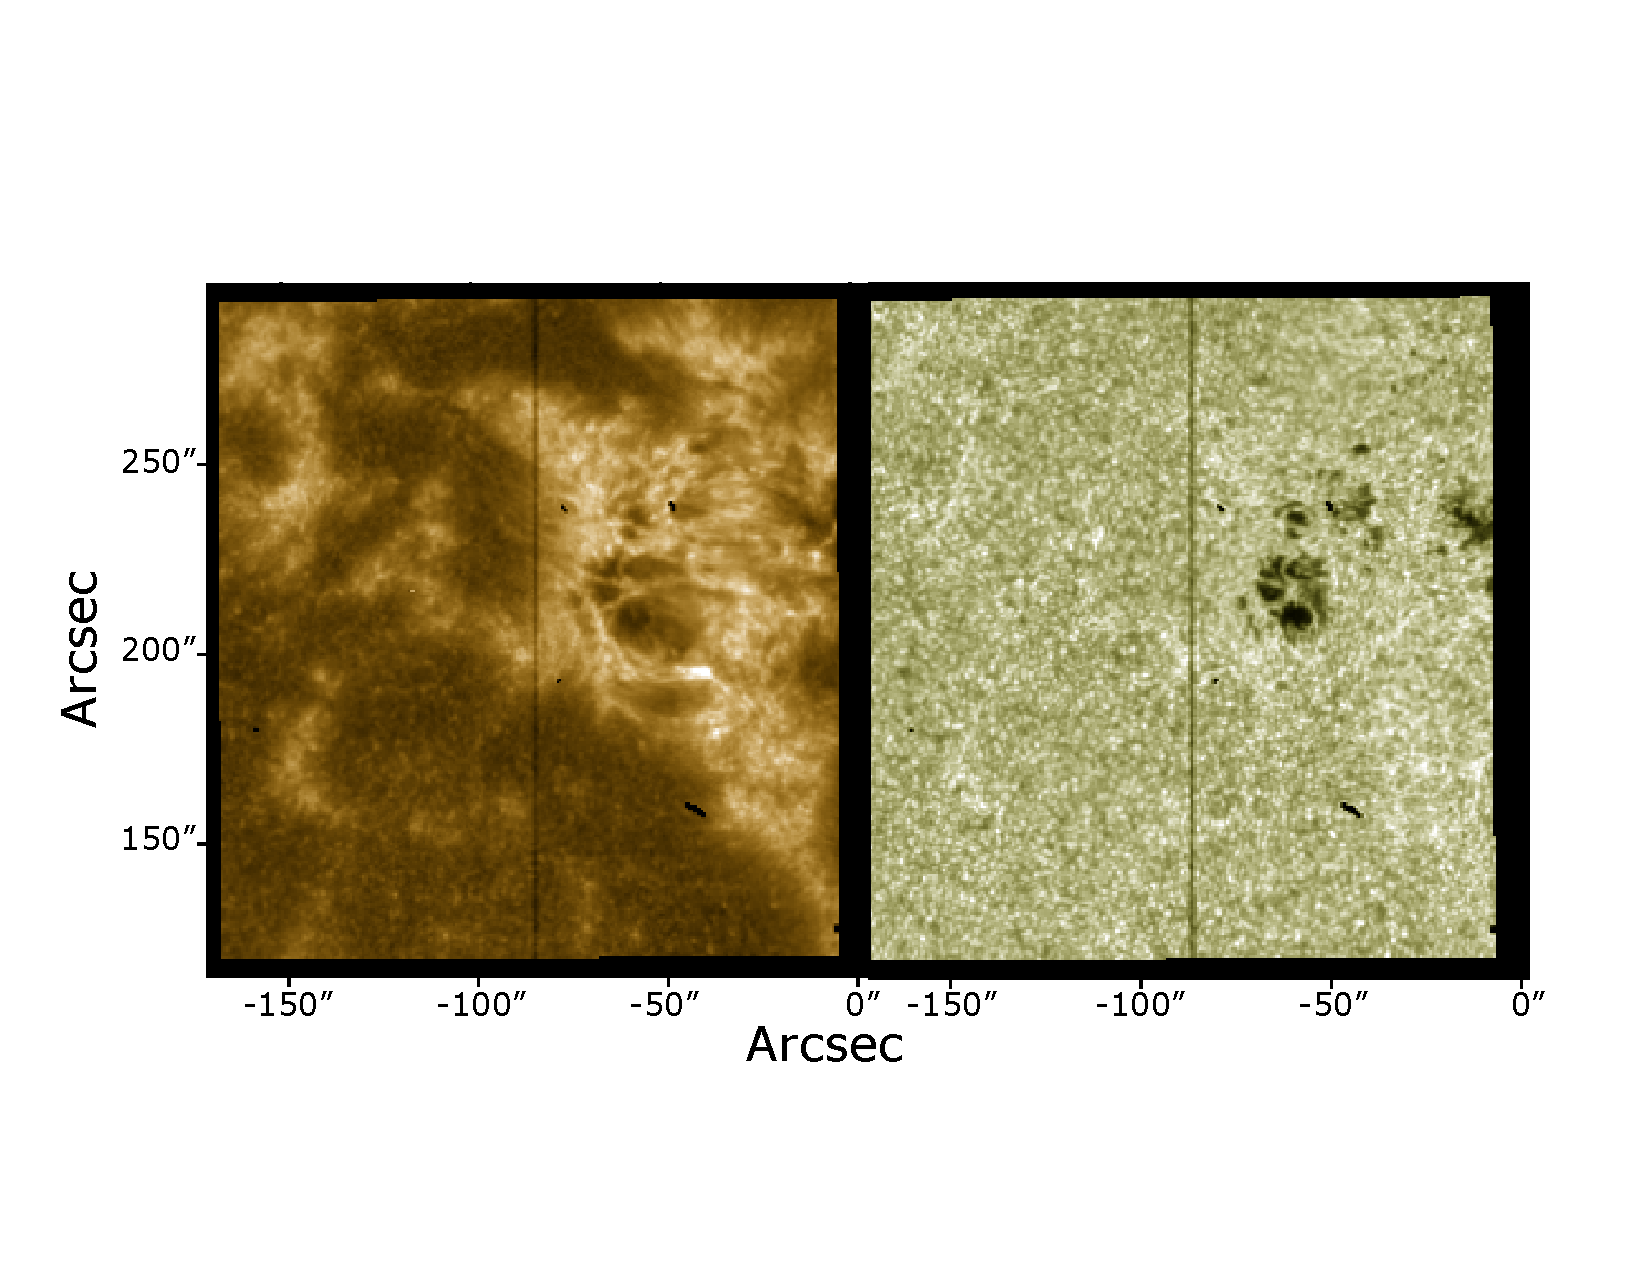
\includegraphics[trim={1cm 3cm 2cm 5cm},clip,width=0.95\textwidth]{Figures/sji_images.pdf}
    \caption[IRIS SJI observation of NOAA AR 13521 on Dec 21st, 2023.]{IRIS slit-jaw images of NOAA AR 13521 taken in \ion{Mg}{2} 2796 {\AA} (left panel) and 2832 {\AA}~continuum (right panel) showing the upper chromosphere and upper photosphere, respectively. Different features are labelled.} 
    \label{fig:sji_features}
\end{figure}
%%%%%%%%%%%%%%%%

%%%%%%%%%%%%%%%%%%%%%%%%%%%%%%%%%%%%%%%%%%%%%%%%%%%%%%%%%%%%%%%%%%%
\subsection{The Transition Region}\label{transition-region}
%%%%%%%%%%%%%%%%%%%%%%%%%%%%%%%%%%%%%%%%%%%%%%%%%%%%%%%%%%%%%%%%%%%

The transition region above the chromosphere is a thin, dynamic layer where we witness a dramatic increase in temperature by two orders of magnitude along with a similar decrease in electron density, demonstrated in Fig.~\ref{fig_solar_atm}. In general, this layer is roughly $\sim$100~km in thickness, but that can change depending on various dynamic conditions of chromosphere ($\sim~10^{4}~K$) below, and corona ($\sim~10^{6}~K$) on top. The transition region is generally characterized by steep changes in temperature, pressure gradients, local optical depth, and competition between gas and magnetic pressure. The transition region also manifests the ARs as various magnetic features such as small-scale brightening, jets, spicules, fibrils etc. 

%%%%%%%%%%%%%%%%%%%%%%%%%%%%%%%%%%%%%%%%%%%%%%%%%%%%%%%%%%%%%%%%%%%
\subsection{The Corona}\label{corona}
%%%%%%%%%%%%%%%%%%%%%%%%%%%%%%%%%%%%%%%%%%%%%%%%%%%%%%%%%%%%%%%%%%%

The outermost layer of the atmosphere is the corona. The corona maintains a temperature of 1-2~MK during ambient conditions but can rise up to tens of MK during explosive eruptions such as solar flares. Due to such high temperatures, the coronal gas is fully ionized. It is only visible to the naked eye during the total solar eclipse or with coronagraphs due to Thomson scattering of the photospheric visible photons with free electrons in the corona. Corona also emits in various emission lines of e.g. Mg, Fe, Si, S, Ca, O, etc. and their ions, across a wide band of electromagnetic spectrum ranging from X-ray to visible wavelengths. Similar to the other layers, the corona exhibits a variety of structures such as ARs, coronal holes, bright points, filaments, and flares. The flare arcades are most prominently visible in the corona. %\info{I made a lot of changes in this section. please see if all is consistent.}

%%%%%%%%%%%%%
\begin{figure}[ht!]
    \centering
    \includegraphics[width=\textwidth]{Figures/aia_features.pdf}
    \caption[Different parts of a flare eruption observed across various wavelengths]{AIA observations of prominence eruption and associated flare as observed on Aug 31st, 2012$\sim$19:50 UT. Different features across different wavelengths have been labelled.}
    %\caption[Different parts of a flare eruption observed across various wavelengths.]{Image of the prominence eruption and associated flare from NOAA AR 11562 on Aug 31st, 2012$\sim$19:50 UT. The prominence is visible in all of the AIA channels. We see the coronal holes in AIA 335 \AA~\textbf{(panel c)}. The flare loops of the associated event is visible in AIA 94 \AA~\textbf{(panel e)} and AIA 131 \AA~\textbf{(panel f)}. The Sunspots are visible in HMI continuum \textbf{panel (h)}. We show a co aligned map of AIA 304 \AA, HMI magnetogram and AIA 131 \AA~in \textbf{panel (i)}. The spatial association of the Sunspots with the hot flareloop plasma and the prominence eruption is clearly demonstrated here. }
    \label{fig:aia-feature}
\end{figure}
%%%%%%%%%%%%%

%\info{I would write the caption of Fig.~\ref{fig:aia-feature} as: AIA observations of prominence eruption and associated flare as observed on Aug 31st, 2012$\sim$19:50 UT. Different features have been labelled.}


%%%%%%%%%%%%%%%%%%%%%%%%%%%%%%%%%%%%%%%%%%%%
\section{Solar Flares}\label{sol_flr}
%%%%%%%%%%%%%%%%%%%%%%%%%%%%%%%%%%%%%%%%%%%%

solar flares are the most powerful energetic explosions in the solar system. They are described as a sudden increase in brightness in localized areas of the Sun. Within tens of minutes, they can release over $10^{32}$ erg of energy, which is emitted across the entire electromagnetic spectrum, i.e., from radio to gamma rays. They can also launch highly energetic particles into the interplanetary medium. Flares occur in magnetic active regions. It has been estimated that the amount of flare energy released is comparable to the free energy stored in the magnetic system \citep{emslie12,ash17}. The total energy released varies from event to event. It is also known that larger events occur much less frequently than smaller events.

Fig.~\ref{fig:sji_features} displays one of the most well-known and well-studied solar eruptions from Aug 31st, 2012. During this event, an associated giant prominence erupted from the southeast limb, which was visible in all AIA channels as shown in Fig.~\ref{fig:aia-feature}. The sunspots are also clearly visible and labelled in the HMI continuum (see Fig.~\ref{fig:aia-feature}h). In Fig.~\ref{fig:aia-feature}i, we show the co-aligned AIA 304 {\AA} and HMI continuum observation. The prominences are rooted at the sunspot penumbra, accompanied by the hot thermal plasma associated with the accompanying flare (visible in Fig.~\ref{fig:aia-feature} e {--} f). The novelty of such observation lies in the clear spatial connection across various layers of the Sun, connected via energy and momentum transported from one layer to the other.

%------------------------------------
\subsection{Brief history of flare observation}\label{sol_flr_1}
%------------------------------------

On September 1, 1859, R.C. Carrington and R. Hodgson independently observed the first flare in white-light continuum \citep{carrington1859, hodgson1859}. Such localized brightening on the Sun has remained an enigma ever since. Shortly after the observation by Carrington and Hodgson, the Sun was being studied extensively in the H$\alpha$ wavelength, which essentially images the chromosphere, and the reports of flaring events became increasingly frequent and progressively more complex. No two events were similar, as there were variations observed in the size of the source, ejections of plasma, and shock waves driving into the interplanetary space. Advances in radio technology during the Second World War affirmed the detection of the presence of non-thermal electrons in the solar corona during military radar operations \citep{hey46}. Around the same time, S.E. Forbrush noticed ground-level cosmic ray enhancement during major solar flares. These discoveries eluded that the flaring events do not only involve the thermal plasma but somehow connect with high energy particles and involve the corona. 

In the late 1950s, using rockets and balloons, the Sun was observed in hard X-rays ($\ge10~keV$). \cite{peterson59} discovered the first hard X-ray emission during a flare in 1958. Later on, it was deduced from the enhancements observed in radio and hard X-rays that the ejected energetic particles may contain a substantial fraction of the initial energy released \citep{brown71}. Note that while the hard X-ray is created by the bremsstrahlung radiation of the electrons colliding into dense material, resulting in a power-law energy distribution, the broadband radio emission from 1 to 100 GHz is created from gyrosynchrotron emission. Flares are now routinely observed with different space-borne instruments, in particular in the EUV and soft X-ray($\le$~10~keV), which shows that the energy released from the flare heats the local plasma to temperatures beyond 30~MK.

%% ################################################################# %%
%\subsection{Neupert effect}\label{npt_eff} \info{I would not give it a name of new subsection}
%% ################################################################# %%

\cite{neupert68} observed a curious correlation that the soft X-ray flux during the rising phase of the flare is proportional to the time integral of the centimetre radio flux since the start of the flare, suggesting a correlation between thermal plasma and the energetic electrons. Note that the centimetre radio flux is emitted by relativistic electrons. A similar correlation was found between the hard X-ray and soft X-ray flux later on. Such correlation can be expressed as,

%%%%%%%%%%%%%%%%%%%%%%%%%%%%%%%%
\begin{equation}\label{npt_eff_eq}
    F_{SXR}(t)~\propto~\int_{t_{0}}^{t}~F_{HXR}(t')~dt'
\end{equation}
%%%%%%%%%%%%%%%%%%%%%%%%%%%%%%%%

\noindent and is known as the ``Neupert effect''. This relationship shows that the soft X-ray radiation primarily originates from a thermal plasma which is heated by the energy of the flaring event deposited by the accelerated electrons. We note, however, that Eqn.~\ref{npt_eff_eq} is only valid if cooling by conduction is negligible and/or the role of ions in the flare energy deposition is minimal \citep{veronig05}.

%% ################################################################# %%
\subsection{``Standard'' model of solar flare}\label{sol_flr_std_mod}
%% ################################################################# %%

Based on various multi-wavelength studies of solar flares, combined with theoretical modelling a `standard' model of solar flares has been advocated by \cite{carmichael64,sturrock66,hirayama74,kopp76}, and termed as \textsl{CSHKP} model. The flares occur due to the abrupt release of magnetic free energy, which was previously stored in the coronal magnetic field via flux emergence and surface motions \citep{forbes06}. The majority of the strongest flares are eruptive in nature. The `standard' model attributes the release of flare energy to magnetic reconnection in the corona, which happens due to the eruption and/or coronal mass ejection \citep{shibata95,lin_n_forbes00,moore01,priest_n_forbes02}. It is noteworthy that, despite continuous attempts over the decades, this is not at all a quantitative model. Rather, it is an attempt to unify the multi-wavelength observations and modelling attempts in an orderly manner. Naturally, the model can not explain all the observations from various flares. A schematic picture of the model is shown in Fig.~\ref{fig:std_mod}. Below we describe the salient points of the `standard' model:

%%%%%%%%%%%%%%%%%%%%%%%%%%%%%%%%%%
\begin{figure}[ht!]
    \centering
    \hspace{5cm}
    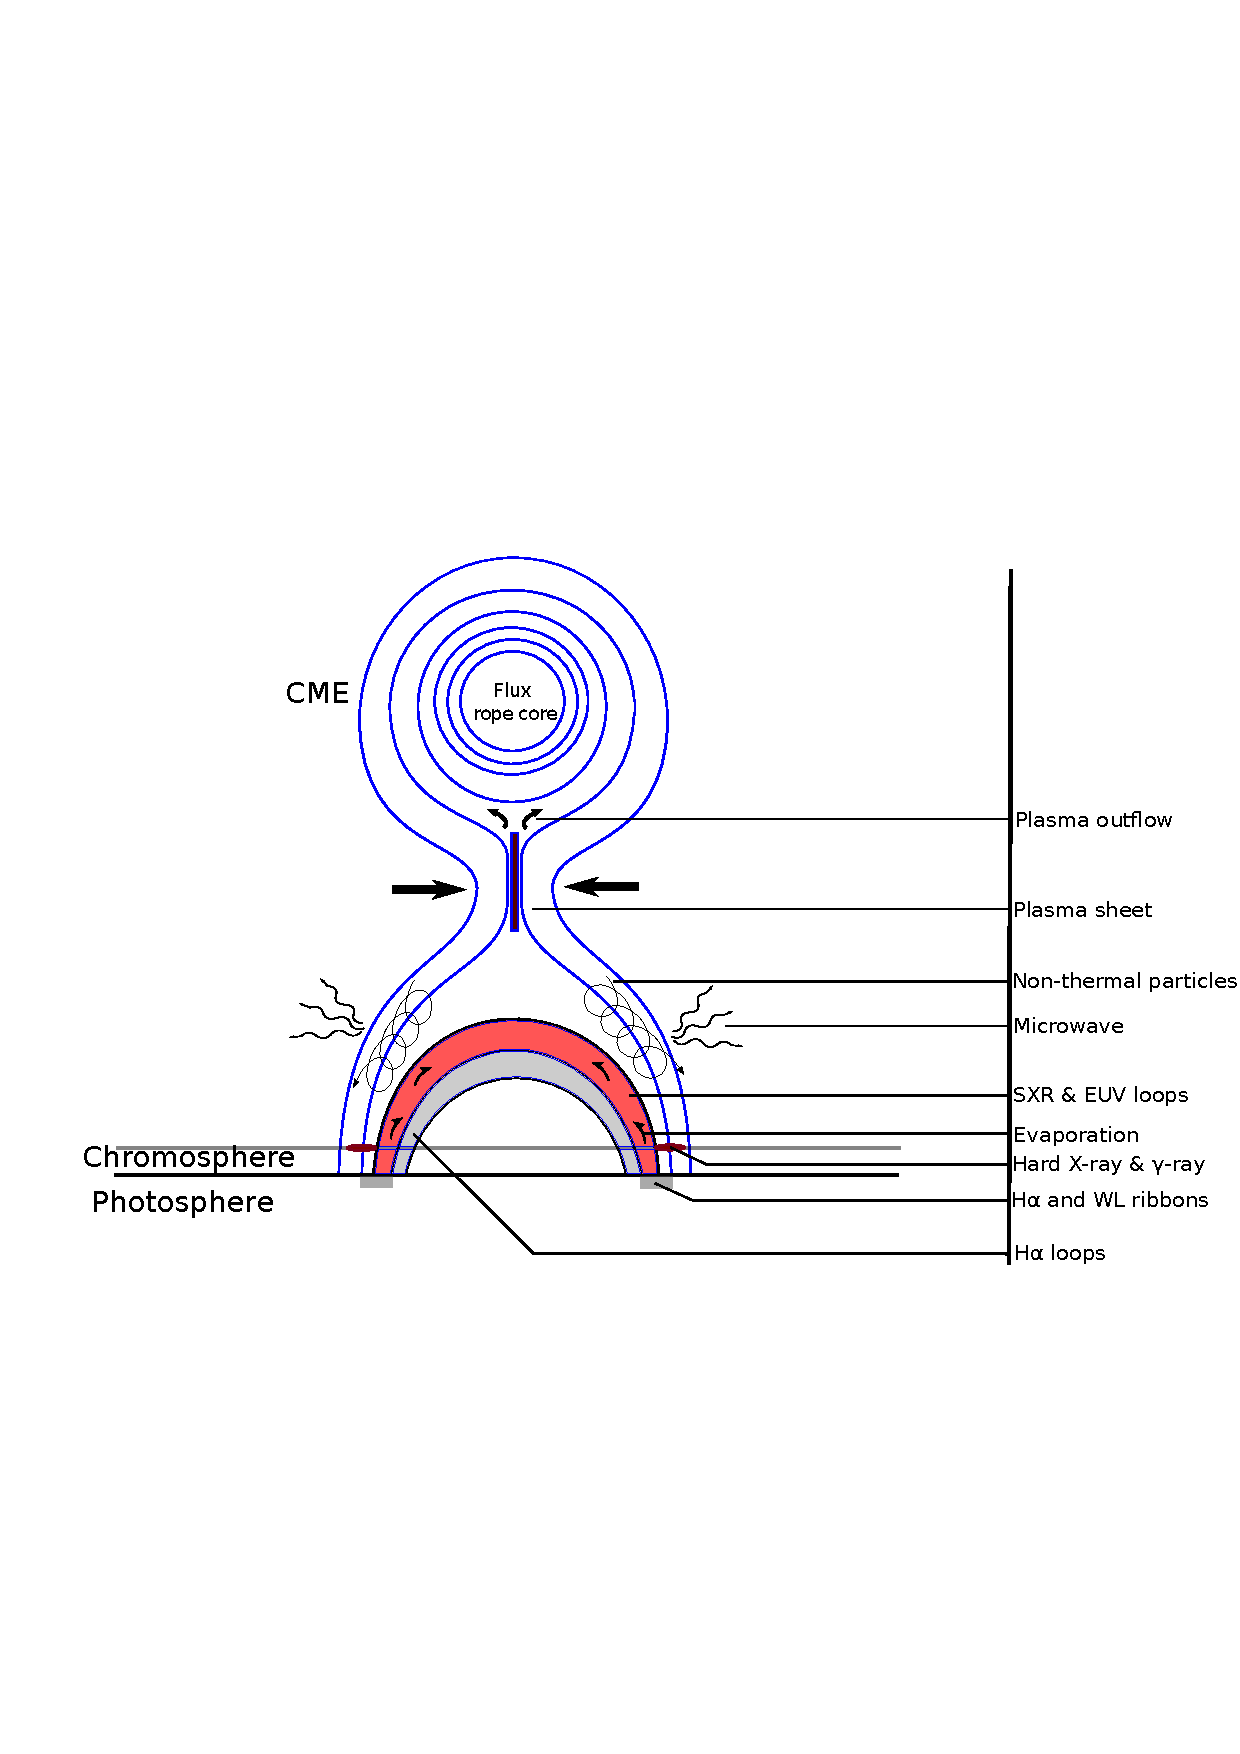
\includegraphics[trim={1cm 8cm 0cm 8cm}, clip, width=0.95\linewidth]{Figures/std_mod.pdf}
    \caption{A schematic diagram of the standard model of solar flare.}
    \label{fig:std_mod}
\end{figure}
%%%%%%%%%%%%%%%%%%%%%%%%%%%%%%%%%%

%%%%%%%%%%%%%%%%%

%\info{This whole description of Standard Model needs to be rewritten. You are going too lateral. Here, the aim is not to bring out the caveats, etc, but to outline the standard model. As you say that you are giving the salient features... so just provide that! Not more than 2-3 sentences in each bullet.}

%\begin{enumerate}
    %\item In the standard model, following the reconnection event occurring that releases the magnetic free energy, electrons and ions from the reconnection site are accelerated along the realigned magnetic field lines. The accelerated particles that escape along the open \info{field lines do not open during flares! Please read Aly and Sturocck paper on this! Very interesting concept!} field lines towards the Earth give rise to the particle events seen from Earth \info{which particles are you talking about? There are different kinds of particles -- particles accelerated due to shock waves that come very fast ... remember proton showers on the detector and other particles which are frozen in the field... they come later}. The coronal reconnection source where the energy is released is often observed in HXR. The loop-top HXR \info{are these same as the reconnection source?} sources are often accompanied by the thermal SXR sources. The loop top HXR source is observed above the coronal SXR source \citep{masuda94}. Later on, most of the HXR sources were reported to be cospatial with the SXR source \citep{bataglia_n_benz07}. This thermal source is distinctly different from the post-flare SXR and EUV loops. This thermal coronal source appears before the HXR emission begins, completely contrary to the "Neupert" behaviour. This SXR loop top source is a key behaviour of the pre-flare phase. The emission measure of these sources is higher than typical coronal levels, suggesting evaporation from the chromosphere before the HXR emission. This also suggests that during the early phases of a flare, the energy is conducted gradually by thermal particles, compared to the energetic non-thermal particles later on.
    
    %Given the existence of the thermal source, the coronal non-thermal source can be explained by a beam of non-thermal particles injected into the dense coronal thermal source. Some of the injected electrons escape the coronal source and precipitate lower. This model is known as the intermediate thin-thick target model (ITTT, proposed by \cite{wheatland95} and investigated further by \cite{metclaf99,fletcher98}.) While the ITTT model explains most of the observations from flares there are certain inconsistencies regarding the coronal X-ray source {\it e.g.} the source of coronal SXR in preflare conditions, difference in expected HXR brightness of the cornal source from models to observations still elude us. It is fair to summarise that even though we by and large understand under what ambient conditions how the coronal HXR source is created, we do not understand what underlying process cause such an environment to arise.
    
    %\item The precipitated particles move along the field lines downwards along the magnetic field lines, giving rise to the microwave and radio observations seen from flares via gyro magnetic radiation at various frequencies dictated by the characteristics of local plasma.
    
    %\item The accelerated particles hit the chromosphere, which is considerably denser than the corona, giving rise to Hard X-ray and gamma-ray observed from the foot points. This also explains why the coronal hard X-ray source is considerably softer than the foot points. The energetic particles deposit their energy into the local chromosphere as they go through a series of collisions and eventually thermalize \citep{brown83}. \sroy{Foot point sources are occasionally detected on H-alpha flare ribbons that are approximately 30,000 km apart, marking the base of a magnetic arcade \citep{masuda01}.}

    %\sroy{$\gamma$-ray emission is visible between 0.8 {--} 20 MeV generated by the accelerated ions. The neutron capture line at 2.2 MeV forming Deuterium is usually the strongest characteristic line visible from such emissions. Protons and other accelerated ions collide with the dense chromosphere and produce neutrons. These neutrons are captured by ambient protons to form Deuteron \citep{ramtay74,hua87}. There were later RHESSI observations \citep{hurford_2003,hurford_2006} that showed that the $\gamma$-ray footpoints did not coincide with the HXR footpoints. This demonstrated that the ions and electrons were accelerated differently, as proposed by \cite{emslie_2004}.}
    %\item  As the plasma thermalizes, it emits in thermal bremsstrahlung, giving rise to the soft X-ray \sroy{radiation}. Also, as the energy is deposited into the chromosphere from the accelerated particles, it heats the local chromosphere environment it gradually increases the local pressure. As the pressure grows, when the pressure gradient builds up enough, the local plasma starts expanding upwards(essentially due to buoyancy) and slowly fills up the coronal loops with soft X-ray emitting plasma. This phenomenon is known as "Chromospheric evaporation". This was directly observed in blue-shifted lines of hot material. \sroy{This was first reported by \cite{doscheck80,feldman80}. \cite{antonucci89} reported velocities of 300 {--} 400 km/s with temperature $\sim$ 20 MK in \ion{Ca}{19}, while later on \cite{milligan06} reported much gentler up-flow with velocities $\sim$ 200 km/s in \ion{Fe}{19} line from {\it SOHO}/CDS observations. Several simulations also reproduced evaporation arising from non-thermal particle precipitation \citep{sterling93,hori98,reeves07}.}
    %\item This whole scenario explains the Neupert effect. As the energy form the accelerated particles is converted into the soft X-ray emitting plasma, and it builds up over time. That explains the soft X-ray being proportional to the time integral of the hard X-ray flux.
%\end{enumerate}
%%%%%%%%%%%%%%%%%

%%%%%%%%%%%%%%%%%
\begin{enumerate}
    \item In the standard model, following the reconnection event that releases the magnetic free energy, electrons and ions from the reconnection site are accelerated along the realigned magnetic field lines downwards. In the case of an associated CME, parts of the magnetic energy is deposited as kinetic energy. The coronal reconnection source where the energy is released is often observed in HXR. The loop-top HXR sources are often accompanied by the thermal SXR sources. The loop top HXR source is observed above the coronal SXR source \citep{masuda94}.
    
    \item The accelerated particles move along the field lines downwards along the magnetic field lines, giving rise to the microwave and radio observations seen from flares via gyro magnetic radiation at various frequencies dictated by the characteristics of local plasma. Finally, the accelerated particles hit the chromosphere, which is considerably denser than the corona, giving rise to Hard X-rays and sometimes also gamma-rays observed from the foot points. This also explains why the coronal hard X-ray source is considerably softer than the foot points. The energetic particles deposit their energy into the local chromosphere as they go through a series of collisions and eventually thermalize \citep{brown83}. Foot point sources are occasionally detected on H-alpha flare ribbons marking the base of a magnetic arcade \citep{masuda01}. The ribbon brightening is usually observed to propagate along the ribbons while they separate further from each other, signifying continued reconnection \citep{tripathi06}.
 
    \item $\gamma$-ray emission from solar flares is visible between 0.8 {--} 20 MeV generated by the accelerated ions. The neutron capture line at 2.2 MeV forming Deuterium is usually the strongest characteristic line visible from such emissions. Flare-accelerated protons and ions colliding with the dense chromosphere can produce neutrons. It is suggested that these neutrons are captured by ambient protons to form Deuteron, giving rise to the 2.2 MeV characteristic bump \citep{ramtay74,hua87}. Later, RHESSI observations \citep{hurford_2003,hurford_2006} showed that the $\gamma$-ray foot-points did not coincide with the HXR foot-points. This demonstrated that the ions and electrons were accelerated differently, as proposed by \cite{emslie_2004}.

    \item  The thermalized plasma emits in thermal bremsstrahlung, giving rise to soft X-ray and EUV radiation. The heating of the local chromosphere increases the local pressure. When the growing pressure gradient builds up enough, the local plasma expands upwards and fills up the coronal loops with soft X-ray-emitting plasma. This phenomenon is known as "chromospheric evaporation". This was first reported by \cite{doscheck80,feldman80}. \cite{antonucci89} reported velocities of 300 {--} 400 km/s with temperature $\sim$ 20 MK in \ion{Ca}{19}, while later on \cite{milligan06} reported much gentler up-flow with velocities $\sim$ 200 km/s in \ion{Fe}{19} line from {\it SOHO}/CDS observations. Several simulations also reproduced evaporation arising from non-thermal particle precipitation \citep{sterling93,hori98,reeves07}.
\end{enumerate}
%%%%%%%%%%%%%%%%%

It is important to emphasise that while the standard model attempts to explain and unify various kinds of differences seen from the numerous flares we observe, there are several cases where the standard model cannot explain the observations. For example, there have been observations of flares where the hard X-ray footpoint does not form \citep{veronig02,veronig04}. It is proposed that in these cases, the plasma in the coronal loops is so dense that the accelerated particles pass through enough collisions to thermalize within the flare loops before reaching the chromosphere. In this process, they may defuse the energy more evenly within the loop rather than impulsively dumping it at the base of the loops. Another flare which previously occurred at the same region might explain the denser coronal loops \citep{strong84,bone07}.  

%% ################################################################# %%
\section{Motivation of the thesis: the energetics of solar flares}\label{sol_flr_energ}
%% ################################################################# %%

Given the rich history of flare observations over more than 150 years, we have learnt a lot about their charactershtics and dyamics. However, there are several complexities involved in the physics of solar flares, which are still fully understood. The reconfiguration of the magnetic structures, which almost always involves complex geometry, makes almost all events unique in some sense. Following the reconfiguration of the magnetic field, the released magnetic free energy is transported across various layers of the Sun and converted into various other forms of energy. The overarching conversion of magnetic energy into various forms, i.e., reconnection outflow, particle acceleration, thermal and kinetic energy of chromospheric plasma, etc., has proven incredibly complex to model. In cases where flares are associated with eruptions, e.g., CMEs, there is the added complexity of the kinetic and potential energy of the CMEs, the associated shocks and the kinetic energy of the solar energetic particles.
%Considering how the energy is transformed the magnetic energy of the active region that is released after the reconnection into the reconnection outflow jets, the kinetic energy of escaping particles, the thermal and the kinetic energy of the Chromospheric plasma evaporating, the radiative and conductive losses. In case of the eruptive events, there is the added complexity of the kinetic and potential energy of the CMEs, the energy of the shocks and the kinetic energy of the solar energetic particles. 

To constrain the models of solar flares and the various associated phenomena, detailed quantitative characterization is absolutely necessary. %There have been several studies quantifying the partition between various subsets of the energies. 
The questions which are of particular importance are:

%%%%%%%%%%%%%%%%%%%%%%%%%%%%%%%%%%%%%%%%%%%%%
\begin{itemize}
    \item Do active regions have enough free energy to account for the total energy released in the solar flares and their associated phenomena?
    \item What is the energy partition between flares and CMEs?
    \item Do the non-thermal component of flares have enough energy to completely power the thermal component or an extra energy source is required to power the thermal component?
\end{itemize}
%%%%%%%%%%%%%%%%%%%%%%%%%%%%%%%%%%%%%%%%%%%%%


%%%%%%%%%%%%%%%%%%%%%%%%%%%%%%%%%%%%%%%%%%%%%
%\begin{itemize}
%    \item \textbf{If an active region can have enough free energy to account for the total energy released in the solar flares and/or CMEs.}
%    \item \textbf{What is the energy partition between flares and CMEs.}
%    \item \textbf{If the non-thermal component have enough energy to power up the thermal component.}
%\end{itemize}
%%%%%%%%%%%%%%%%%%%%%%%%%%%%%%%%%%%%%%%%%%%%%

While it is now established the active regions have enough magnetic free energy to power the flare and CME and other associated phenomena  \citep{emslie12,ash17}, the energy partition between the flare and associated CME is much more fuzzy. \cite{emslie12} found that the flare and CME have energies of the same order of magnitude, while \cite{ash17} concluded the energy in the flare dominates that of the associated CME. 

The question about the non-thermal component having sufficient energy to power the thermal component is still unresolved, as even the most recent studies contradict each other in the most puzzling fashion. \cite{warmuth20} discussed the contradictions arising from some of the studies~\citep{stosire07,emslie12,inglis14,warmuth16a,warmuth16b,ash17}, the details of which are summarized in Table~\ref{tab1}.

%%%%%%%%%%%%%%%%%%%%%%%%%%%%%%%%%%%%%%%%%%%%%%%
\begin{table}[ht!]
    \centering
    \resizebox{\textwidth}{!}{%
    \begin{tabular}{||c|c|c|c|c|c|c||}
    \hline 
    \hline
       Study & No. of flares & GOES class range & Thermal model & Thermal spectrum & Thermal volume & Thermal losses \\
       \cite{stosire07} (S07 from hereon) & 18 & A3-B7 & Isotherm. & RHESSI & TRACE & X \\
       \cite{emslie12} (E12 from hereon) & 38 & C5-X28 & Isotherm. & RHESSI & RHESSI & Rad. \\
       \cite{inglis14} (IC14 from hereon) & 10 & B3-B9 & Multitherm. & RHESSI+AIA & RHESSI & Rad. \\
       \cite{warmuth16a,warmuth16b} (WM16 from here on) & 24 & C3-X17 & Isotherm. & RHESSI+GOES & RHESSI & Rad.,Cond. \\
       \cite{ash17} (A17 from here on) & 188 & M1-X7 & Multitherm. & AIA & AIA & Rad. \\
       \hline
    \end{tabular}}
    \caption{Observational summary of the flares as described in \cite{warmuth20}.}
    \label{tab1}
\end{table}
%%%%%%%%%%%%%%%%%%%%%%%%%%%%%%%%%%%%%%%%%%%%%%%

The bolometric energy serves as a representation of the overall energy released during solar flares. Regardless of the mechanism of energy release, e.g., through direct plasma heating, rapid bulk flows, or non-thermal particles, etc., the ultimate outcome is the thermalization of the plasma and the subsequent radiation. Since the bolometric energy encompasses the entire electromagnetic spectrum, it reflects the total energy originally of the flare. Note, however, that this bolometric energy only pertains to the energy liberated within the flare and does not include the energy associated with the concurrent CME. %\cite{warmuth20} used the bolometric energy released in solar flares to compare various studies on equal footing. Here we will discuss some of the main issues \cite{warmuth20} identifies comparing these studies.

Fig.~\ref{fig:goes-therm} displays correlation plots between peak thermal energy and peak GOES flux (left panel) for various flares studied by various authors and corresponding (where available) volume estimates of the thermal plasma (right panel). The plots show that the estimated thermal energy obtained in all studies shows an excellent correlation with peak {\it GOES} flux. Also plotted are the bolometric energies obtained by \cite{emslie12, kretzschmar11}. %Fig.~\ref{fig:goes-therm} left panel shows the peak thermal energy as a function of peak {\it GOES} flux for all the flares from the five studies. 
Note that the thermal energy obtained by E12 (open red diamonds) and WM16 (filled black circles) are consistently one order of magnitude lower than the bolometric energy (open green diamonds and solid green line) of flares with similar peak GOES flux. Extrapolation of E12 and WM16 is about half an order of magnitude lower compared to IC14 (open blue triangles), while S07 (open pink flipped triangles) is very consistent with the extrapolation. Note that the energies estimated in A17 (orange plus signs) are about an order of magnitude higher than that obtained in other studies and even higher than the extrapolated bolometric energy for flares of the same class from \cite{kretzschmar11} and E12. 

The above described results present a contradiction in the results obtained in different studies. While there could be several reasons for these differences, they can be attributed to differences in modelling the thermal component of the flares. For example, {\it RHESSI} usually yields a higher temperature and lower emission measure compared to {\it GOES} due to the highly multi-thermal nature of the flaring plasma \citep{bataglia05,ryan14,warmuth16a}. Although the {\it GOES} temperature is higher by a factor of 1.4, it is not dependent on the flare class. Moreover, \cite{warmuth20} also investigated whether assuming an isothermal or multi-thermal model introduces any differences in the thermal energy estimates. They reported no significant differences due to differences in models (refer to Fig.2 and the corresponding discussion in \cite{warmuth20}). Notably, these comparisons of isothermal and models are made by fitting spectra obtained by spatially binning spectra. This does not really incorporate the multithermal nature of the plasma varying spatially.

%%%%%%%%%%%%%%%%%%%%%%%%%%%%%%%%%%%%%%%%%%%%%%%
\begin{figure}[ht!]
    \centering
    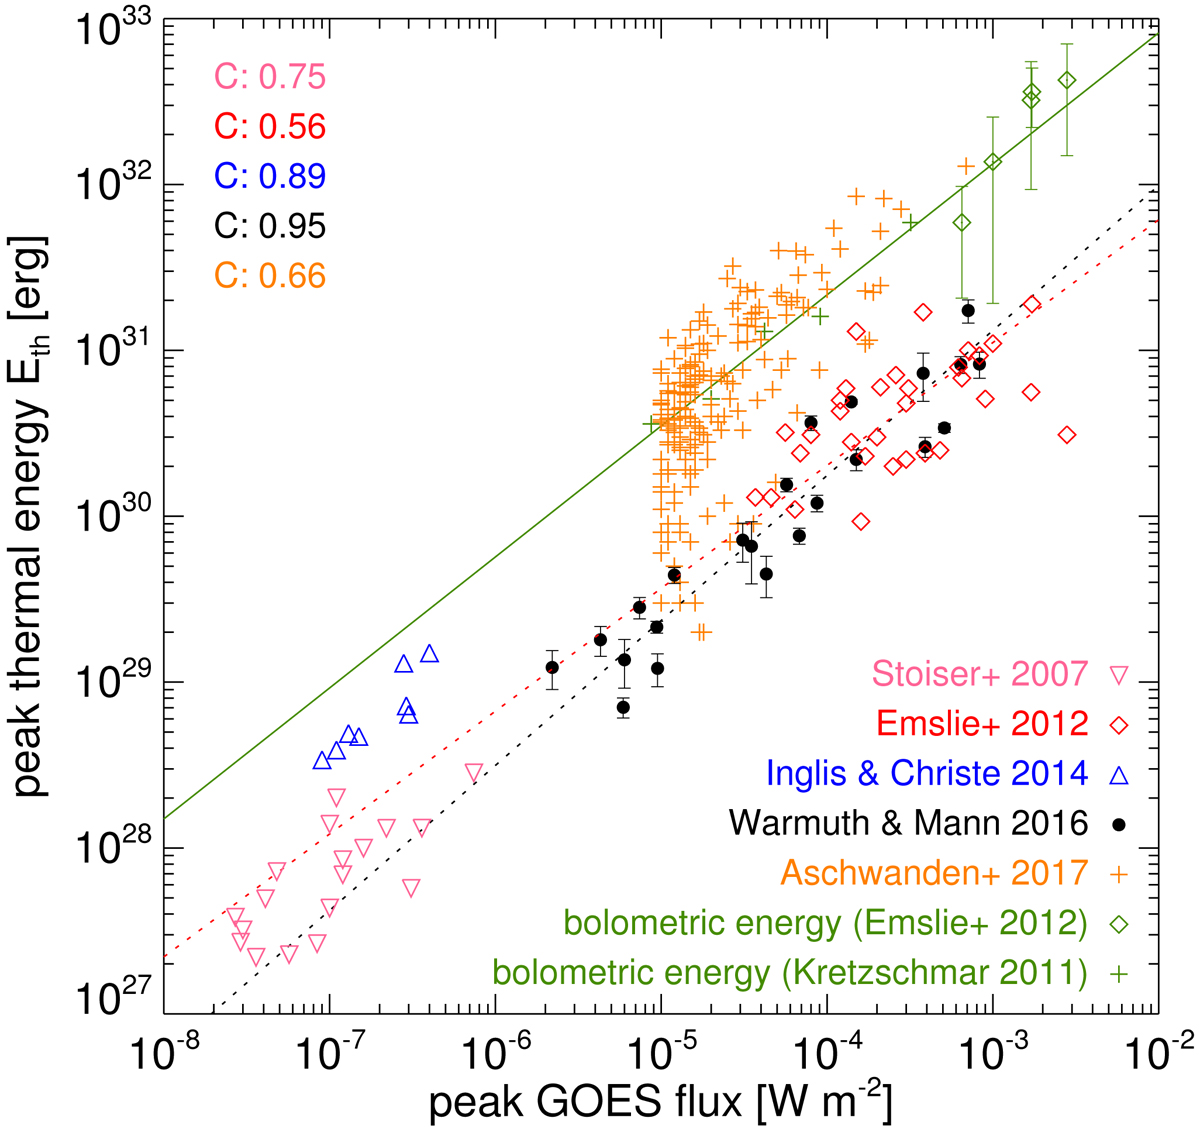
\includegraphics[width=0.49\textwidth,trim={0cm 0cm 0cm 0.02cm},clip]{goes_flux_therm.jpg}
    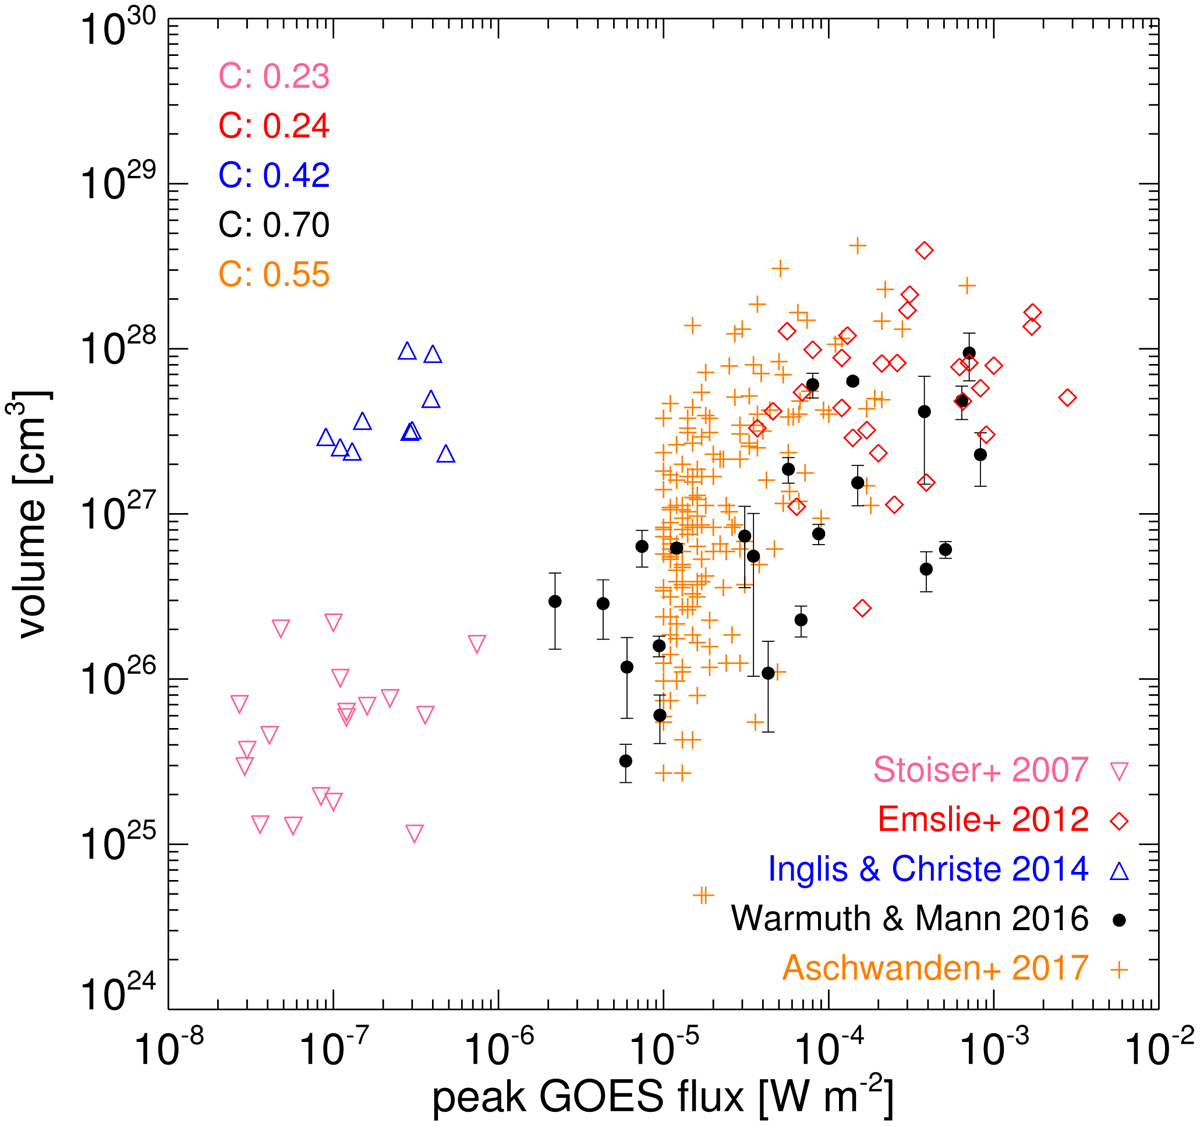
\includegraphics[width=0.49\textwidth,trim={0cm 0cm 0cm 0.02cm},clip]{goes_flux_vol.jpg}
    \caption[Correlation of peak {\it GOES} flux with peak thermal energy and flaring plasma volume.]{{\it GOES} peak thermal energy (left panel) and volume of the thermal plasma (right panel) as a function of the peak {\it GOES} flux for all the flares from five studies (figure credit: \cite{warmuth20}). The C values show the linear correlation coefficient for various studies.}
    \label{fig:goes-therm}
\end{figure}
%%%%%%%%%%%%%%%%%%%%%%%%%%%%%%%%%%%%%%%%%%%%%%%

The thermal energy is estimated using $$\mathrm{U_{Th}\sim n_{e}k_{B}TVf}$$
\noindent where n$_e$ is the electron density, k$_B$ is Boltzmann's constant, T is the temperature, V is the volume of the flaring plasma, and f is the filling factor.

 Fig.~\ref{fig:goes-therm} right panel shows the volumes used for various studies to estimate the thermal energy as a function of the peak {\it GOES} flux. Apart from S07 and A17, all other studies used {\it RHESSI} imaging to estimate the flare volume with a filling factor $f=1$. S07 determined the volume by employing a semicircular loop model, utilizing the cross-sectional area and loop length derived from the observed areas and separations of foot point brightening of 1600  {\AA} by {\it TRACE}. In contrast, A17 estimated the volume based on the flare area exceeding a certain threshold in the emission measure obtained from the spatial synthesis DEM method. 

It is worth noting that the volume estimates from E12 and WM16 align closely, as do those from A+17, despite employing entirely different methodologies. In contrast, the micro flare volumes reported by IC14 are notably larger, ranging from one to two orders of magnitude beyond what would be anticipated based on the findings of the other four studies. Intriguingly, this discrepancy aligns with the additional volume required to account for the higher thermal energies observed in IC14. The uncertainty in detecting volume can be due to the CLEAN (Component Least Squares Deconvolution) algorithm systematically overestimating the source size \citep{warmuth13a}. There have also been studies demonstrating that {\it RHESSI} has difficulties in resolving small sources \citep{dennis09,warmuth13b}, that would be applicable for small thermal sources in the microflares. %This illustrates the requirement for better volume estimation for better estimates of the thermal energy of flares.

From the above-described studies, it is clear that there are number of questions that are crucial to describe the physics of solar flares. We allude to these below. 

%We can conclude a few more puzzling questions from these studies as a whole: %\info{These are not questions but more like statements. Please make them questions.}

%--------------------------------------------------------------------
\begin{itemize}
    \item The primary challenge in estimating the thermal energy of the hot plasma stems from determining the temperature distribution of the plasma using Differential Emission Measure (DEM), and the radiating plasma volume. How strongly do the uncertainties of determining the thermal energy depend on the uncertainties of the volume estimation and the highly mutithermal nature of the flaring plasma? 
    \item The dissipation of energy from the hot plasma is substantial. Although there is widespread agreement regarding radiative losses across studies, the extent of conductive losses disagree significantly between the studies. Why do various studies vary so significantly on the extent of conductive losses across the literature and what effect does it have on the thermal evolution of the flares?
    \item How much do the non-thermal energy in injected electrons depend on the poorly constrained low-energy cutoff?
    \item The thermal and non-thermal energy partition changes with flare class. In smaller flares, there appears to be a deficiency of energetic electrons, whereas in larger flares, the injected non-thermal energy seems to be sufficient in powering the thermal component. Does this signify the existence of an additional third heating source?
\end{itemize}
%--------------------------------------------------------------------

In the limited scope of this thesis address the following pressing questions through multiwavelength observations and contribution in the development of new instruments:
%--------------------------------------------------------------------
\begin{itemize}
\item How does the thermal and non-thermal energy partition change over the duration of flares? What effect do the uncertainties of volume estimation have, on the thermal energy estimates and what conclusions can we draw from that regarding the tension in the thermal and non-thermal energy sources?

\item Flares connect various layers of the solar atmosphere via different mechanisms during various stages of its evolution. How does the signature of flares look in the NUV regime which mainly originate in the photosphere, chromosphere and transition region. The transition region is one of the least observed part of the solar atmosphere in context of flares. What is the spectral energy distribution of flares across various wavelength regime and layers, specifically in NUV?
\end{itemize}
%--------------------------------------------------------------------

%\info{I would also suggest that you use this section to identifiy all the questions that you are going address in the thesis... partition between thermal and non-thermal is one, other is NUV radiation in flare etc...}

%In addition to these, there is one more looming question, related to the "standard" model of flares itself, that has been largely unanswered, not due to lack of efforts, rather limited mostly by the technological limitations dictating the detectability of the current instruments. In \S\ref{sol_flr_std_mod}, we discussed about the fundamental differences inferred between the acceleration mechanisms of electrons and ions inferred from the different locations of the HXR and $\gamma$-ray foot points. The production of $\gamma$-ray from nuclear reactions in chromosphere opens up the possibility of high-energy nuclear reactions producing pions ($\pi^{0}$ and $\pi^{\pm}$) along with secondary neutrinos ($\nu$) through the decay of the pions. Such reactions would be driven by protons with energy $>$ 300 MeV \citep{ramtay75,hudson_n_ryan_95}. Detection of neutrinos will open up a new window in constraining the effects of the accelerated particles in the lower solar atmosphere, i.e., chromosphere and photosphere and the general characteristics of the local plasma environment. Unfortunately, in spite of considerable efforts no flare neutrinos have been detected so far. It is understood that the first hurdle is to detect a minute transient signal on top of the large solar neutrino background. This informs our required detection thresholds driven by the current ion acceleration models \citep{sol_nu_kamiokande,abe_2022}. If the inability to detect flare neutrinos persists, it indicates that not enough protons/ions with energies $>$ 300 MeV is produced even in very large flares. That would impose an upper limit of the amount of energy that is deposited in particle acceleration from flaring events and/or the efficiency of the acceleration mechanism. \info{this discussion is good here but not necessary. I leave it to you to decide!}

%--------------------------------------------------------------------
%\section{Motivation}\label{sec:mot}. 
%--------------------------------------------------------------------
%\info{This section is what we shall use as the synopsis. So, it should have : 1 st para: What are flares and why are they important. 2nd para: what is know and what is missing (only the most important aspects). 3rd Para: what is the overall goal, and what extra do you do? Just briefly. Thereafter Chapter wise summary.}

%The main motivation of this thesis is to add understanding of effects of flares on the surrounding environment in lower and upper solar atmosphere, to answer some of the questions posed above. We have used imaging and spectroscopic observations from multiple space based observatories, e.g., AIA, HMI, IRIS, XRT, etc. This research contributes to creating a perspective of flare energetics and its effect on the surrounding plasma environment from chromosphere to corona. \info{again written with Capital C...}

%The solar flares are the strongest magnetic event in our solar system connecting various layers of the solar atmosphere ({\it e.g.} from photosphere to corona), coupled via mass and energy transport. While the coronal manifestation of solar flares has been studied extensively with several instruments, there are only a few imaging and spectroscopic instruments observing the photosphere to transition region. These include the {\it IRIS} \citep{iris}, AIA 1600, 1700, and 304~{\AA} \citep{aia} and some other filters of {\it Hinode}/SOT \citep{sot}. In addition to these, we also have had balloon experiment {\it SunRISE} \citep{Sunrise1,Sunrise2}, which provided high-resolution imaging of the chromosphere, from the SuFI instrument \citep{sufi}. \textbf{where are you using Sunrise?}

%This illustrates the necessity of more observatories operating at the chromospheric wavelengths for a more comprehensive understanding of how the solar flares manifest and affect the dynamics and heating of the lower solar atmosphere. More specifically, there is a gap in understanding the spectral energy distribution of flares and the flare signatures in NUV arising from the chromosphere and photosphere. 

%The main motivation of this thesis is to add an understanding of the effects of flares on the surrounding environment in the lower and upper solar atmosphere to answer some of the questions posed in \S\ref{sol_flr_energ}. We have used imaging and spectroscopic observations from multiple space-based observatories, e.g., AIA, HMI, IRIS, XRT, etc. This research contributes to creating a perspective of flare energetics and its effect on the surrounding plasma environment from the chromosphere to the corona.

%\info{Shouldn't the above two paragraphs swapped?}


%This illustrates the necessity of more observatories operating at the transition region \info{There is a lot of upper transition region data e.g., 171, what is missing is chromosphere. SUIT does not observe transition region} wavelengths for more comprehensive understanding about how the solar flares manifest and affect the dynamics and heating of the lower solar atmosphere. In this regard, {\suit} onboard Aditya-L1 will play a crucial role in probing the lower solar atmosphere. The various imaging channels of {\suit} would observe the manifestation of flares in transition region at various heights (NB3 $\implies$ \ion{Mg}{2} k 279.6 nm, NB4 $\implies$ \ion{Mg}{2} h 280.3 nm, NB8 $\implies$ \ion{Ca}{2} h 396.8 nm), further lower in the transition region (NB2 $\implies$ blue wing of Mg window, NB5 $\implies$ red wing of Mg window) and Sunspots and possible signature of umbral brightening due to flares at the photosphere (NB6 300 nm and NB7 388 nm) in full disk. This would also allow us to probe the interaction of the flaring region, with other active regions on disk, giving us a comprehensive overview of the effect of solar flares and their manifestation in the lower solar atmosphere.

%% ################################################################# %%
\section{Outline of Thesis}\label{sec:outline}
%% ################################################################# %%


This thesis primarily focuses on studies of solar flares and their signatures in various layers of the solar atmosphere by using multi-wavelength observation and contribution to the development of the solar Ultraviolet Imaging Telescope (SUIT) on board the Aditya-L1 mission. The rest of the thesis is structured as follows: 

%%%%%%%%%%%%%%%%%%%%%%%%%%%
\begin{itemize} 
	
	\item Chapter~\ref{c:chap2}: To perform various studies in this thesis, we have used observations from several instruments. Moreover, we have used several techniques to analyse the data and derive physical parameters from these observations. Therefore, we dedicate this chapter to providing relevant details of each instrument we have used. Moreover, we discuss the analysis techniques by providing relevant details and salient features. We emphasise the {\suit} instrument, mention its primary science goals, and briefly discuss the specific questions that {\suit} can address regarding solar flares.
	
	\item Chapter~\ref{c:chap3}: This chapter addresses the partition between solar flares' thermal and non-thermal energy and their time evolution in two flares. For this purpose, we use multi-wavelength observations from two vantage points recorded by {\it SDO}/AIA, {\it STEREO-A}/EUVI, {\it SO}/STIX, {\it GOES}/SUVI. Using existing tools and the observations from two vantage points, we propose a new method to accurately calculate the volume of the flaring plasma, which is a crucial parameter in the derivation of thermal energy. We demonstrate that an accurate estimate of the volume of flaring plasma as a function of time can affect the accurate estimation of thermal energy and, therefore, will have significant implications on the partition between the thermal and non-thermal energy components.
	
	\item Chapter~\ref{c:chap4}: Here we discuss some of the initial preparatory analysis we performed for {\suit} instrument, including the throughput model, selection of science filters, modelling of the spacecraft jitter and its effects on the imaging performance of the instrument. We also describe a scheme for absolute calibration using standard stars like Vega and Sirius. For this purpose, we have used Sun-as-a-star spectra combined with the instrument's throughput model to evaluate the calibration scheme.
	
	\item Chapter~\ref{c:chap5}: Having derived the instrument model for SUIT, we now forward the model to the expected observations the instrument will record.  For this purpose, we use MPS-Atlas simulation and {\it IRIS} observations, with measured transmission profiles of various optical components and the PSF.
	
	
	\item Chapter~\ref{c:chap6}: The two filters, among 11, that SUIT has are tuned to observe the Mg~\Romannum{2}~h~\&~k lines. Therefore, in preparation for SUIT, we study three flares belonging to three different classes, namely X, M and C, observed by IRIS in spectroscopy mode. We study the ratio of the two spectral lines \textit{viz.}, Mg~\Romannum{2}~h~\&~k for the three flares. The ratio of the Mg \Romannum{2}~k\&~h lines is a proxy for the optical depth of the surrounding plasma. We found that the line intensity ratio shows a correlated increase and decrease with the flare light curve. We argue this to be the signature of plasma flow associated with flare and a change in the density of the local environment. %Such studies could b This acts as a prelude of what is achievable with {\suit}. We can use a similar method to give full disk context of optical depth with respect to eruptive events.
	
	\item Chapter~\ref{c:chap7}: The SUIT instrument was switched on Nov 20th, 2023, while still in the cruise phase, with a first light on December 6th. The spacecraft was inserted into the halo orbit around L1 point on Jan 06, 2024. Since the first light, it has detected several flares, both with and without getting into flare mode. In this Chapter, we discuss the first flare observed on Feb 22, 2024, after enabling the flare detection algorithm. We discuss the first results and show the capabilities of the SUIT instrument for flare physics.

    \item Chapter~\ref{c:chap8}: Finally, we summarize the results obtained in the various projects in the context of the overarching perspective of flare energetics and its signature in the chromosphere and photosphere in NUV. We also discuss the caveats and the eventual progression of these projects, as well as the future prospects.
	
	
	% and what new questions they open up. Moreover, we also discuss the likely required observations to address the questions regarding flares and which questions they would address.
   % \item In chapter \ref{c:chap7} we discuss the first flare observations of {\suit}. What do you find? 
\end{itemize}
%%%%%%%%%%%%%%%%%%%%%%%%%%


%\listoftodos
%%%%%%%%%%%%%%%%%%%%%%%%%%%